\documentclass[11pt, spanish, a4paper, twopage]{article}

% Versión 1.er cuat 2021 Víctor Bettachini < vbettachini@unlam.edu.ar >

\usepackage[T1]{fontenc}
\usepackage[utf8]{inputenc}

\usepackage[spanish, es-tabla]{babel}
\def\spanishoptions{argentina} % Was macht dass?
% \usepackage{babelbib}
% \selectbiblanguage{spanish}
% \addto\shorthandsspanish{\spanishdeactivate{~<>}}

\usepackage{graphicx}
\graphicspath{{./figuras/}{../LaTeX/}}
% \usepackage{float}

\usepackage[arrowdel]{physics}
\newcommand{\pvec}[1]{\vec{#1}\mkern2mu\vphantom{#1}}
% \usepackage{units}
\usepackage[separate-uncertainty= true, multi-part-units= single, range-units= single, range-phrase= {~a~}, locale= FR]{siunitx}
\usepackage{isotope} % $\isotope[A][Z]{X}\to\isotope[A-4][Z-2]{Y}+\isotope[4][2]{\alpha}

\usepackage{tasks}
\usepackage[inline]{enumitem}
% \usepackage{enumerate}

\usepackage{hyperref}

% \usepackage{amsmath}
% \usepackage{amstext}
% \usepackage{amssymb}

\usepackage{tikz}
\usepackage{tikz-dimline}
\usetikzlibrary{calc}
% \usetikzlibrary{math}
\usetikzlibrary{arrows.meta}
\usetikzlibrary{snakes}
\usetikzlibrary{decorations}
\usetikzlibrary{decorations.pathmorphing}
\usetikzlibrary{patterns}

\usepackage[hmargin=1cm,vmargin=3cm, top= 0.75cm,nohead]{geometry}

\usepackage{lastpage}
\usepackage{fancyhdr}
\pagestyle{fancyplain}
\fancyhf{}
\setlength\headheight{28.7pt} 
\fancyhead[LE, LO]{\textbf{Mecánica General} }
\fancyhead[RE, RO]{\href{https://ingenieria.unlam.edu.ar/}{$\vcenter{\hbox{
\includegraphics[height=1cm]{ambos.pdf}}}$}}
\fancyfoot{\href{https://creativecommons.org/licenses/by-nc-sa/4.0/deed.es_ES}{$\vcenter{\hbox{
\includegraphics[height=0.4cm]{by-nc-sa_80x15.pdf}}}$} \href{https://ingenieria.unlam.edu.ar/}{DIIT - UNLaM}}
\fancyfoot[C]{ {\tiny Actualizado al \today} }
\fancyfoot[RO, LE]{Pág. \thepage/\pageref{LastPage}}
\renewcommand{\headrulewidth}{0pt}
\renewcommand{\footrulewidth}{0pt}


\begin{document}
\begin{center}
	% \textsc{\large Mecánica general}\\
	\textsc{\large Vibraciones en sistemas discretos | Múltiples grados de libertad}
\end{center}

% De poder resolver estos problemas en forma autónoma puede asumir que adquirió los conocimientos mínimos sobre los temas abordados en la semana. No dude en consultar a docentes y compañeros si no puede terminarlos. Los problemas marcados con * son opcionales.

\begin{enumerate}

				
\item 
\begin{minipage}[t][4cm]{0.65\textwidth}
En el sistema de la figura \(l = \SI{0.5}{\metre}\), \(k_1 = k_2 = k = \SI{2E3}{\newton\per\metre}\) y \(m_1 = m_2 = m_3 = m = \SI{1}{\kilo\gram}\).
Asumiendo pequeñas las oscilaciones en torno al cero de las coordenadas indicadas:
\begin{tasks}
	\task obtenga las ecuaciones de Euler-Lagrange,
	\task escríbalas en forma matricial (matrices M, K), y
	\task obtenga las frecuencias naturales de oscilación del sistema.
\end{tasks}
\end{minipage}
\begin{minipage}[c][0cm][t]{0.3\textwidth}
	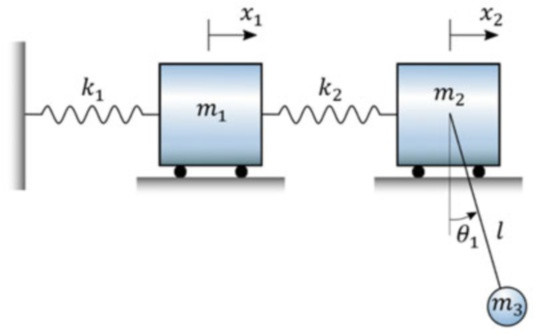
\includegraphics[width=\textwidth]{shabana_fig_P3_6.png}
\end{minipage}



\item 
\begin{minipage}[t][2.5cm]{0.65\textwidth}
\textbf{Péndulo de torsión compuesto}

El sistema de la figura consiste en un eje atraviesa tres discos que tienen por momentos de inercia \(I_1, I_2\) e \(I_3\) todos de igual magnitud \SI{1E3}{\kilo\gram\metre\squared}.
El eje de acero tiene un diámetro \(d = \SI{0.01}{\metre}\) y sus secciones longitudes de \(l_1 = l_2 = l_3 = \SI{0.5}{\metre}\).
\end{minipage}
\begin{minipage}[c][1cm][t]{0.3\textwidth}
	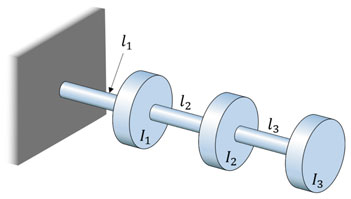
\includegraphics[width=\textwidth]{shabana_fig_P3_5.png}
\end{minipage}


Recordemos que para una coordenada angular \(\theta\) la ecuación de Euler-Lagrange es
\[
	\Gamma \dot{\theta} + \kappa \theta + I \ddot{\theta} = \tau,
\]
donde \(\Gamma\) en la fricción torsional, \(I\) el momento de inercia, \(\tau\) el torque aplicado.
$\kappa$ es la \href{https://es.wikipedia.org/wiki/Resorte_de_torsi%C3%B3n#Coeficiente_de_torsi%C3%B3n}{rigidez torsional (torsional stiffness) o coeficiente de torsión} que responde al torque restitutivo que ejerce la pieza al ser torcida en un ángulo unidad, $\tau_\text{restitutivo} = - \kappa \theta$ y su magnitud la determina 
\[
	\kappa = \frac{G J}{l},
\]
donde \(l\) es la longitud de la pieza, \(G\) el \href{https://es.wikipedia.org/wiki/M%C3%B3dulo_de_cizalladura}{módulo de cilladura (shear modulus)} específico de cada material, y \(J\) es el \href{https://es.wikipedia.org/wiki/Módulo_de_torsión}{módulo o momento de torsión} de la sección geométrica transversal a la dirección de $\vec{\tau}$.
Para una sección circular \(J\) es igual al segundo momento del área, o \href{https://es.wikipedia.org/wiki/Segundo_momento_de_%C3%A1rea}{momento de inercia polar}
\[
	J_{zz} = J_{xx} + J_{yy} = \frac{\pi r^4}{2} = \frac{\pi d^4}{32}.
\]
Según el documento \href{https://tsapps.nist.gov/publication/get_pdf.cfm?pub_id=101021}{Mechanical Properties of Structural Steels} publicado por National Institute of Standards and Technology estadounidense, para el acero estructural de las \href{https://es.wikipedia.org/wiki/World_Trade_Center_(1973-2001)}{torres 1 y 2 del World Trade Center de Nueva York desaparecidas el año 2001},
\[
	\begin{aligned}
		G &= g_0 + g_1 T + g_2 T^2 + g_3 T^3 + g_4 T^4 + g_5 T^5\\
		g_0 &= \SI{80.005922}{\giga\pascal}\\
		g_1 &= \SI{-0.018303811}{\giga\pascal\per\celsius}\\
		g_2 &= \SI{-1.5650288E-5}{\giga\pascal\per\celsius\tothe{2}}\\
		g_3 &= \SI{-1.5160921E-8}{\giga\pascal\per\celsius\tothe{3}}\\
		g_4 &= \SI{-1.6242911E-11}{\giga\pascal\per\celsius\tothe{4}}\\
		g_5 &= \SI{7.7277543E-15}{\giga\pascal\per\celsius\tothe{5}}
	\end{aligned}
\]

Descartando la fricción rotacional \(\Gamma\):
\begin{tasks}
	\task obtenga las ecuaciones de Euler-Lagrange,
	\task escríbalas en forma matricial (matrices M, K), y
	\task obtenga las frecuencias naturales de oscilación del sistema.
\end{tasks}



\end{enumerate}
\end{document}
